\documentclass[12pt]{article}

\usepackage{amsmath, amsfonts, amssymb}
\usepackage[margin=0.5in]{geometry}
\usepackage{graphicx}
\graphicspath{ {./Figures/} }

\title{Tychonoff Theorem}
\author{Kyle Jiang}
\date{05/29/2024}

\begin{document}

\maketitle


Here, we will prove the \emph{Tychonoff Theorem}, which states

\textbf{Tychonoff Theorem. } Arbitrary products of compact spaces are compact.

\vspace{1 \baselineskip}

Recall the definition of \emph{compactness}:

\textbf{Definition. } A space $X$ is \emph{compact} if, for every open cover $\mathcal{C}$ of $X$, there exists a finite subcollection $\{ C_1, \dots, C_N \} \subseteq \mathcal{C}$ that covers $X$.

\vspace{1 \baselineskip}

We begin with the following lemma, which formulates compactness in terms of closed sets.

\textbf{Lemma. } A space $X$ is compact if and only if for each collection $\mathcal{A}$ of closed sets with the finite intersection property (FIP), $\bigcap \mathcal{A}$ is nonempty.

We say that a collection of subsets $\mathcal{A}$ has the \emph{finite intersection property} (FIP) if any finite subcollection $\{ A_1, \dots, A_N \}$ has a nonempty intersection.

\textbf{Proof. } ($\implies$) Let $X$ be compact. Let $\mathcal{A}$ be a collection of closed subsets of $X$ such that $\mathcal{A}$ has the FIP. Suppose for the sake of contradiction that $\bigcap \mathcal{A}$ is empty. Consider the collection $\mathcal{C} = \{ X - A | A \in \mathcal{A} \}$; note that each element of $\mathcal{C}$ is open. Furthermore, by deMorgan's Laws, we know that

$$\emptyset = \bigcap \mathcal{A} = \bigcap_{C \in \mathcal{C}} (X - C) = X - \bigcup \mathcal{C}$$

$$\implies \bigcup \mathcal{C} = X$$

In other words, $\mathcal{C}$ is an open cover of $X$. By hypothesis, $\mathcal{C}$ contains a finite subcollection $\{ C_1, \dots, C_N \}$ that covers $X$. Now, again by deMorgan, we have that

$$X = C_1 \cup \dots \cup C_N = X - [(X - C_1) \cap \dots \cap (X - C_N)]$$

$$\implies \emptyset = (X - C_1) \cap \dots \cap (X - C_N)$$

Each $X - C_i$ is an element of $\mathcal{A}$ by construction. Therefore, the finite subcollection $\{ X - C_1, \dots, X - C_N \}$ of $\mathcal{A}$ has empty intersection, which contradicts the hypothesis that $\mathcal{A}$ has the FIP.

($\impliedby$) Suppose $X$ is such that that for each collection $\mathcal{A}$ of closed sets with the FIP, $\bigcap \mathcal{A}$ is nonempty. By contrapositive, if $\mathcal{A}$ is a collection of closed sets such that $\bigcap \mathcal{A}$ is empty, then $\mathcal{A}$ does not have the FIP; i.e., $\mathcal{A}$ contains some finite subcollection $\{ A_1, \dots, A_N \}$ whose intersection is empty. Let $\mathcal{C}$ be an arbitrary open cover of $X$. Consider the collection of closed sets given by $\mathcal{A} = \{ X - C | C \in \mathcal{C} \}$. By deMorgan's Laws,

$$\bigcap \mathcal{A} = \bigcap_{C \in \mathcal{C}} (X - C) = X - \bigcup \mathcal{C} = X - X = \emptyset$$

so that $\mathcal{A}$ does not have the FIP. Then $\mathcal{A}$ contains some finite subcollection $\{ A_1, \dots, A_N \}$ whose intersection is empty. The subcollection $\{ X - A_1, \dots, X - A_N \}$ of $\mathcal{C}$ covers $X$.

\vspace{1 \baselineskip}

With this lemma in place, we are now in a position to understand the Tychonoff theorem. Let $\{ X_\alpha \}_{\alpha \in J}$ be a family of compact spaces. We wish to show that the space $Y = \prod_{\alpha \in J} X_\alpha$ is compact. Based on the lemma just proven, it suffices to show that for any collection $\mathcal{A}$ of closed sets of $Y$ that satisfies the FIP, the intersection $\bigcap \mathcal{A}$ is nonempty.

We might initially approach this as follows. Let $\mathcal{A}$ satisfy the hypothesis. Select, for each $\alpha \in J$, a point $x_\alpha \in X_\alpha$ such that $x_\alpha \in \bigcap_{A \in \mathcal{A}} \text{Cl} \pi_\alpha (A)$, which is possible because $X_\alpha$ is compact. (Recall that $\pi_\alpha: Y \to X_\alpha$ is the projection map.) We would hope that $(x_\alpha) \in \bigcap \mathcal{A}$, which would complete the proof. However, this is not necessarily the case, as the following simple counterexample shows.

\textbf{Example. } Consider the product $Y = X_1 \times X_2$, where $X_1 = X_2 = [0, 1]$, with $Y \subseteq \mathbb{R}^2$. Take $\mathcal{A}$ to be the collection of closed rectangles oriented diagonally as follows:

\begin{center}
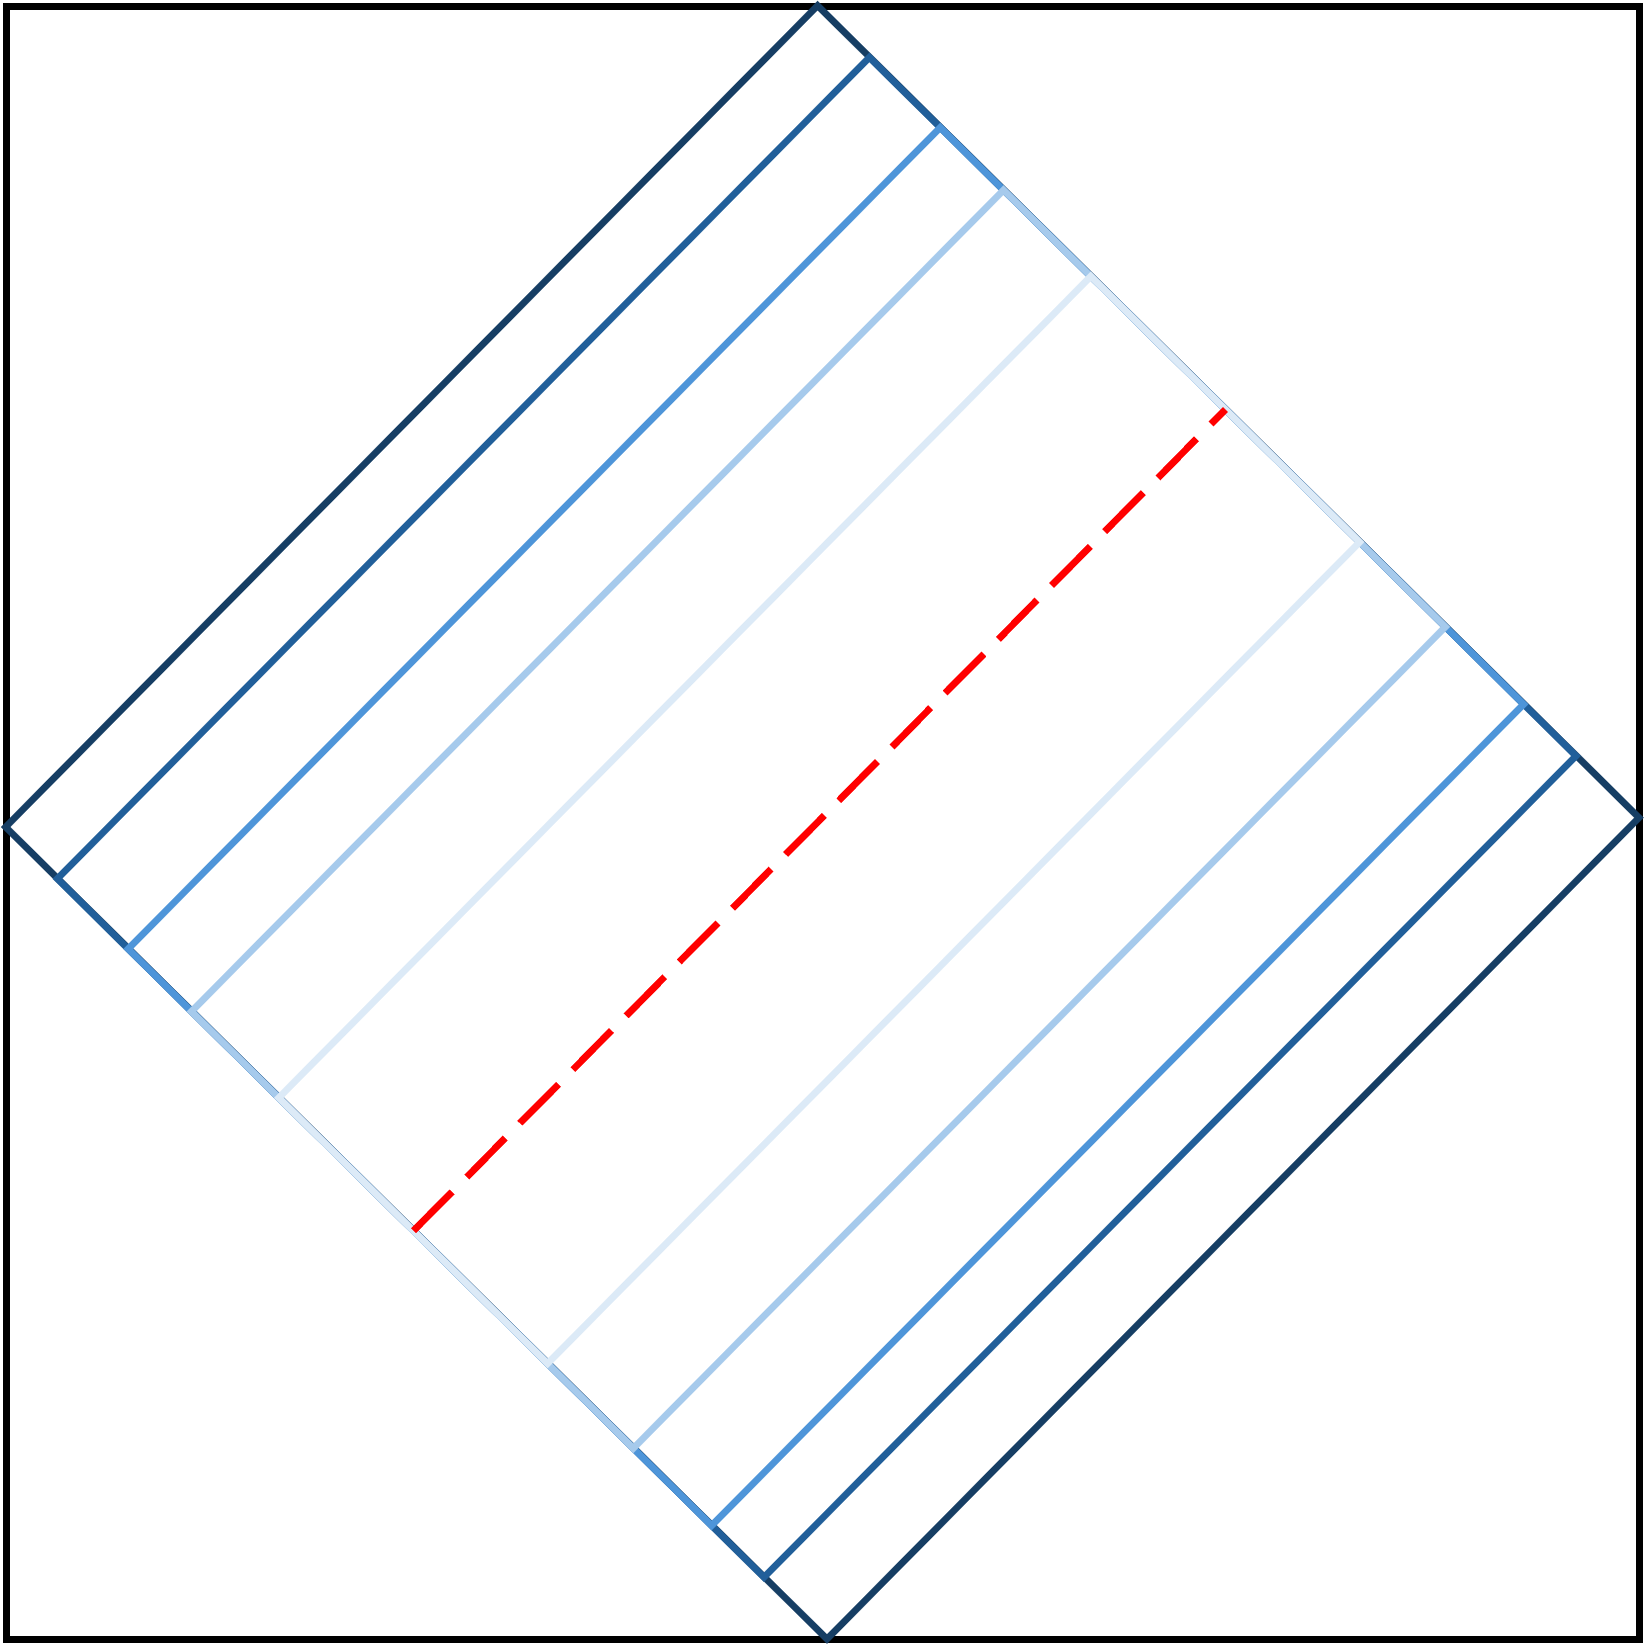
\includegraphics[width=4in]{./tut_tychonoff_1.png}
\end{center}

Clearly, $\mathcal{A}$ satisfies the FIP, since it is a nested sequence of nonempty sets. And, the intersection $\bigcap \mathcal{A} = \left\{ x \times x | x \in \left[ \frac{1}{4}, \frac{3}{4} \right] \right\}$, denoted by the dashed red line, is nonempty.

Let's consider the process of finding an element in $\bigcap \mathcal{A}$ as described above. For both factors $\alpha \in \{ 1, 2 \}$ of the product space, we have that $\bigcap_{A \in \mathcal{A}} \text{Cl} \pi_\alpha (A) = \left[ \frac{1}{4}, \frac{3}{4} \right]$. Since the selection of $x_\alpha$ is arbitrary, it would be possible to select, for example, $x_1 = \frac{1}{4}$ and $x_2 = \frac{3}{4}$. But $\frac{1}{4} \times \frac{3}{4} \notin \bigcap \mathcal{A}$.

So, this way of finding a point in $\bigcap \mathcal{A}$ was not sufficient. The insightful idea offered by Tychonoff is to restrict the element of the product that is chosen. In the general case, it is not clear how to do so. When there is not a clear indication of how to construct a set, it is useful to consider \emph{extremal sets}; i.e., a largest or smallest set satisfying certain properties. To prove the Tychonoff theorem, it turns out that letting $\mathcal{D}$ be a collection such that

\begin{enumerate}
\item $\mathcal{A} \subseteq \mathcal{D}$, 
\item $\mathcal{D}$ has the FIP, and
\item $\mathcal{D}$ is not properly contained in any other collection with the previous properties
\end{enumerate}

and then selecting $x_\alpha \in X_\alpha$ such that $x_\alpha \in \bigcap_{D \in \mathcal{D}} \text{Cl} \pi_\alpha (D)$, it is then true that $(x_\alpha) \in \bigcap_{D \in \mathcal{D}} \text{Cl} D \implies (x_\alpha) \in \bigcap \mathcal{A}$. It is said that $\mathcal{D}$ is \emph{maximal} with respect to the FIP.

\vspace{1 \baselineskip}

We must of course first prove that such a $\mathcal{D}$ exists.

\textbf{Proposition. } Such a collection $\mathcal{D}$ as described above exists.

\textbf{Proof. } Consider the collection $\mathbb{B}$ of all collections $\mathcal{B}$ of subsets of $Y$ such that

\begin{enumerate}
\item $\mathcal{A} \subseteq \mathcal{B}$, and
\item $\mathcal{B}$ has the FIP.
\end{enumerate}

To show that $\mathbb{B}$ has a maximal element (with respect to set inclusion), we can use Zorn's Lemma.

(\textbf{Zorn's Lemma. } Suppose a partially ordered set $\mathbb{P}$ has the property that every totally ordered subset of $\mathbb{B}$ has an upper bound in $\mathbb{B}$. Then the set $\mathbb{B}$ contains at least one maximal element.)

Let $\mathbb{C}$ be a totally ordered subset of $\mathbb{B}$ (totally ordered with respect to set inclusion). Then for any $\mathcal{C} \in \mathbb{C}$, it is true that $\mathcal{A} \subseteq \mathcal{C}$, and $\mathcal{C}$ has the FIP. Consider the union $\mathcal{C}^* = \bigcup \mathbb{C}$. We claim that it is contained in $\mathbb{B}$, and that it is an upper bound of $\mathbb{C}$.

($\mathcal{C}^* \in \mathbb{B}$) Let $A \in \mathcal{A}$. Then $A \in \mathcal{C} $ for every $\mathcal{C} \in \mathbb{C}$, so it is obvious that $A \in \mathcal{C}^*$. This shows $\mathcal{A} \subseteq \mathcal{C}^*$. Now, consider any finite collection $\{ C_1, \dots, C_N \} \subseteq \mathcal{C}^*$. For each $i \in \{ 1, \dots, N \}$, select some $\mathcal{C}_i \in \mathbb{C}$ that contains $C_i$. Since $\mathbb{C}$ is totally ordered, and the collection $\{ \mathcal{C}_i \}$ just described is finite, there exists some $i' \in \{ 1, \dots, N \}$ such that $\mathcal{C}_i \subseteq \mathcal{C}_{i'}$ for each $i$. Thefore, $\{ C_1, \dots, C_N \} \subseteq \mathcal{C}_{i'}$, and since $\mathcal{C}_{i'} \in \mathbb{C}$ has the FIP, then the intersection $C_1 \cap \dots \cap C_N$ is nonempty.

($\mathcal{C}^*$ is an upper bound of $\mathbb{C}$) This is trivial.

Since $\mathbb{C}$ was arbitrary, Zorn's Lemma applies to show that $\mathbb{B}$ indeed has a maximal element $\mathcal{D}$, as desired.

\vspace{1 \baselineskip}

The maximality of $\mathcal{D}$ endows it with the following useful properties.

\textbf{Proposition. } $\mathcal{D}$ is closed to finite intersections.

\textbf{Proof. } Let $D_1, D_2 \in \mathcal{D}$, and suppose for the sake of contradiction that $D_3 = D_1 \cap D_2 \notin \mathcal{D}$. Consider the collection $\mathcal{D}' = \mathcal{D} \cup \{ D_3 \}$, which properly contains $\mathcal{D}$. Obviously, $\mathcal{A} \subseteq \mathcal{D} \subseteq \mathcal{D}'$ implies that $\mathcal{A} \subseteq \mathcal{D}'$. Now, consider a finite collection $\{ E_i \}_{i \in \{ 1, \dots, N \}} \subseteq \mathcal{D}'$. If $D_3 \notin \{ E_i \}$, then $\bigcap \{ E_i \}$ is nonempty from the fact that $\mathcal{D}$ satisfies the FIP. If $D_3 \in \{ E_i \}$, then

$$\bigcap \{ E_i \} = \left( \bigcap \{ E_j \ne D_3 | E_j \in \{ E_i \} \} \right) \cap (D_1 \cap D_2)$$

which is still a finite intersection of elements of $\mathcal{D}$ and therefore nonempty. This contradicts the maximality of $\mathcal{D}$.

\vspace{1 \baselineskip}

\textbf{Proposition. } If $D \subseteq Y$ intersects each element of $\mathcal{D}$, then $D \in \mathcal{D}$.

\textbf{Proof. } Let $D$ intersect each element of $\mathcal{D}$, and suppose for the sake of contradiction that $D \notin \mathcal{D}$. Consider the collection $\mathcal{D}' = \mathcal{D} \cup \{ D \}$, which properly contains $\mathcal{D}$. Obviously, $\mathcal{A} \subseteq \mathcal{D} \subseteq \mathcal{D}'$ implies that $\mathcal{A} \subseteq \mathcal{D}'$. Now, consider a finite collection $\{ E_i \}_{i \in \{ 1, \dots, N \}} \subseteq \mathcal{D}'$. If $D \notin \{ E_i \}$, then $\bigcap \{ E_i \}$ is nonempty from the fact that $\mathcal{D}$ satisfies the FIP. If $D \in \{ E_i \}$, then

$$\bigcap \{ E_i \} = \underbrace{\left( \bigcap \{ E_j \ne D | E_j \in \{ E_i \} \} \right)} \cap D$$

The underbraced term above, being a finite intersection of elements of $\mathcal{D}$, is -- by the previous proposition -- an element of $\mathcal{D}$. By hypothesis, each element of $\mathcal{D}$ intersects $D$, so that $\bigcup \{ E_i \}$ is nonempty. This contradicts the maximality of $\mathcal{D}$.

\vspace{1 \baselineskip}

We now use these results to prove the Tychonoff Theorem.

\textbf{Proof of Tychonoff Theorem. } Let $\{ X_\alpha \}_{\alpha \in J}$ be a family of compact spaces, and consider $Y = \prod_{\alpha \in J} X_\alpha$. Let $\mathcal{A}$ be a collection of closed sets in $Y$ such that $\mathcal{A}$ has the FIP. Our results above guarantee a $\mathcal{D}$ containing $\mathcal{A}$ that is maximal with respect to the FIP. (Note that the elements of $\mathcal{D}$ are not required to be closed.) We claim that if the point $(x_\alpha) \in Y$ is such that $x_\alpha \in \bigcap_{D \in \mathcal{D}} \text{Cl} \pi_\alpha (D)$ for each $\alpha \in J$, then $(x_\alpha) \in \bigcap_{D \in \mathcal{D}} \text{Cl} D$. Recall that a point satisfying the premise of this claim always exists because for each $\alpha \in J$,

\begin{itemize}
\item $\{ \text{Cl} \pi_\alpha (D) | D \in \mathbb{\mathcal{D}} \}$ is a collection of closed sets with the FIP, and
\item $X_\alpha$ is compact.
\end{itemize}

Consider an arbitrary subbasis element $V_\alpha = \pi_\alpha^{-1} (U_\alpha) \subseteq Y$, where $U_\alpha$ is a neighborhood of $x_\alpha \in X_\alpha$. Let $D \in \mathcal{D}$ be arbitrary. We know that $x_\alpha \in \text{Cl} \pi_\alpha (D)$. Therefore, $U_\alpha$ intersects $\pi_\alpha (D)$, and $V_\alpha$ intersects $D$. From our results above, this implies $V_\alpha \in \mathcal{D}$.

Now, let $B$ be an arbitrary basis element containing $(x_\alpha)$. By definition, $B$ can be expressed as the finite intersection of subbasis elements, which are all contained in $\mathcal{D}$. Again from our results above, this implies that $B \in \mathcal{D}$.

Given any $D \in \mathcal{D}$, since $\mathcal{D}$ has the FIP, each basis element $B$ containing $(x_\alpha)$ intersects it, implying that $(x_\alpha) \in \text{Cl} D$. Therefore, $(x_\alpha) \in \bigcap_{D \in \mathcal{D}} \text{Cl} D$.

To complete the proof, we simply note that $\mathcal{A} \subseteq \mathcal{D}$ implies that $(x_\alpha) \subseteq \text{Cl} A = A$ for each $A \in \mathcal{A}$. This shows $(x_\alpha) \in \bigcap \mathcal{A}$, as desired.


\vspace{2 \baselineskip}


\textbf{Proposition. } Let $X$ be a space, and $\mathcal{D}$ be a collection of subsets of $X$ that is maximal with respect to the FIP. Then $x \in \text{Cl} D$ for every $D \in \mathcal{D}$ if and only if every neighborhood of $x$ belongs to $\mathcal{D}$.

\textbf{Proof. } ($\implies$) Suppose $x \in \text{Cl} D$ for every $D \in \mathcal{D}$. Let $U$ be an arbitrary neighborhood of $x$, and $D \in \mathcal{D}$ be arbitrary. By hypothesis, $U$ intersects $D$. Therefore, $U$ intersects each element of $\mathcal{D}$. By the maximality of $\mathcal{D}$, $U \in \mathcal{D}$.

($\impliedby$) Suppose every neighborhood of $x$ belongs to $\mathcal{D}$. Let $D \in \mathcal{D}$ be arbitrary. Since $\mathcal{D}$ has the FIP, and $U \in \mathcal{D}$ for each neighborhood $U$ of $x$, $U \cap D$ is nonempty. This shows $x \in \text{Cl} D$.

\vspace{1 \baselineskip}

\textbf{Proposition. } Let $D \in \mathcal{D}$. If $D \subseteq A$, then $A \in \mathcal{D}$.

\textbf{Proof. } Since $\mathcal{D}$ has the FIP, $D$ intersects each element of $\mathcal{D}$. It is easy to check that $A \supseteq D$ does the same. Therefore, by maximality of $\mathcal{D}$, $A \in \mathcal{D}$.

\vspace{1 \baselineskip}

\textbf{Proposition. } If $X$ is Hausdorff, then there is at most one point contained in $\bigcap_{D \in \mathcal{D}} \text{Cl} D$.

\textbf{Proof. } Suppose that $x \in \bigcap_{D \in \mathcal{D}} \text{Cl} D$ and $y \ne x$. Since $X$ is Hausdorff, there exist disjoint neighborhoods $U, V$ of $x, y$, respectively. Since $U$ is a neighborhood of $x$, then by a previous proposition, $U \in \mathcal{D}$. Since $\mathcal{D}$ has the FIP, and $V$ does not intersect $U$, then $V \notin \mathcal{D}$. Since $V$ is a neighborhood of $y$ that does not belong to $\mathcal{D}$, then $y \notin \bigcap_{D \in \mathcal{D}} \text{Cl} D$, by a previous proposition.


\end{document}